% !TeX program = xelatex
\documentclass[12pt]{article}
\usepackage[right=1.0in,left=1.0in,top=1.0in,bottom=1.0in]{geometry}
\usepackage{hyperref}
\hypersetup{colorlinks, citecolor=blue, filecolor=blue, linkcolor=blue, urlcolor=blue}
\usepackage{graphicx}
\usepackage{url}
\usepackage[round]{natbib}
\usepackage{amsmath,amsthm,amssymb}
\usepackage{booktabs}
\usepackage{multirow}
\usepackage{float}
\usepackage{pdflscape}
\usepackage[labelfont=bf,labelsep=period]{caption}
\usepackage{subcaption}
\usepackage{longtable}
\usepackage{threeparttable}
\usepackage{threeparttablex}
\usepackage{environ}

\usepackage{setspace}
\onehalfspacing

\let\textcite\citet

\graphicspath{{../results/figures/}}

% Appendix-style section/table/figure numbering (A.1, A.2, ...)
\renewcommand{\thesection}{\Alph{section}}
\renewcommand{\thetable}{\thesection.\arabic{table}}
\renewcommand{\thefigure}{\thesection.\arabic{figure}}
\renewcommand{\theequation}{\thesection.\arabic{equation}}

%%%%%%%%%%%%%%%%%%%%%%%%%%%%%%%%%%%%%%%%%%%%%%%%%%%%%%%%%%%%%

\title{Medical School Environments and Physician Treatment Styles \\[0.5em]
\large SUPPLEMENTAL APPENDIX}

\author{Shirley Cai\thanks{Emory University.} \and Ian McCarthy\thanks{Emory University.
\href{mailto:ian.mccarthy@emory.edu}{ian.mccarthy@emory.edu}}}

\date{\today}

%%%%%%%%%%%%%%%%%%%%%%%%%%%%%%%%%%%%%%%%%%%%%%%%%%%%%%%%%%%%%

\begin{document}

\maketitle

\section{Sample Construction Details}\label{sec:app-sample}

This section provides additional detail on the construction of our cardiologist-year analytical panel, the medical-school-to-HRR crosswalk, the AHA training-period cath-lab measure, and the NIH ExPORTER ranking panel.

\subsection{Cardiologist Assignment and Volume Restriction}

For each NSTEMI episode, we assign a single attending cardiologist following the procedure of \textcite{molitor2018}. The hierarchy prioritizes the first cardiologist who delivers a consultation (CPT codes 99251--99255 prior to their elimination by CMS in January 2010, with the hierarchy collapsing to first cardiologist of record for inpatient care for episodes thereafter), the first cardiologist of record on the inpatient stay, and the first cardiologist seen by the patient in carrier-line claims within 90 days of the index admission. We exclude episodes for which no cardiologist could be assigned and patient-years for which Medicare fee-for-service coverage was not present for the entire year. Cardiologists are identified in MD-PPAS using primary-specialty fields for cardiology, interventional cardiology, clinical cardiac electrophysiology, and advanced heart failure and transplant cardiology.

We restrict to cardiologist-years with at least 11 NSTEMI patients. The threshold provides stable per-physician estimates of catheterization rates and aligns with the CMS cell-size threshold for public-use files. A trade-off of the volume restriction is that established, higher-volume cardiologists are over-represented in our analytical sample relative to the broader cardiologist population.

\subsection{Residualized Catheterization Rate}

Our outcome is the volume-weighted mean residualized cath-within-two-days indicator at the cardiologist-year level. At the patient level, we estimate a linear probability model regressing the cath-within-two-days indicator on the 31 Elixhauser comorbidity flags and year fixed effects, retaining the residual as the patient-level outcome. We then aggregate to the cardiologist-year by taking the volume-weighted mean residual. The residualization removes mechanical variation across cardiologists that would arise from differences in patient comorbidity mix.

Elixhauser comorbidities are constructed from a lookup table of approximately 2,600 ICD-9 and ICD-10 diagnosis codes mapped to 31 categories, drawn from the cardiologist's NSTEMI-episode and 12-month-look-back claims. A given diagnosis code may map to multiple Elixhauser categories, so the lookup is implemented as a join rather than a categorical recoding.

\subsection{Medical-School-to-HRR Crosswalk}

The medical-school HRR is constructed in three stages. First, we obtain each cardiologist's medical school name and graduation year from the CMS Physician Compare National Downloadable File. Second, we map medical school names to ZIP codes using a hand-curated crosswalk restricted to LCME-accredited U.S. allopathic medical schools, validated against the LCME accreditation directory. Of 187 medical schools in our crosswalk, 186 resolve via the LCME accreditation join, and one historically defunct school resolves via a separate fallback ZIP. Schools coded in Physician Compare as ``OTHER'' are excluded; the OTHER category captures most foreign-trained physicians and a small number of unmatched U.S. schools. Third, we map ZIP codes to hospital referral regions using the Dartmouth Atlas ZIP-to-HRR crosswalk (vintage 2015).

Our analytical panel restricts to allopathic MD graduates because only roughly 11\% of U.S. medical school graduates are osteopathic (DO), with an even smaller share among cardiologists (AAMC, U.S.\ Physician Workforce Data Dashboard).

\subsection{AHA Training-Period Cath-Lab Measure}

Cath-lab availability is recorded in the AHA Annual Survey CCLABHOS variable from 1994 onward and in the predecessor CCLAB82 variable from 1980--1993. Both are recoded to a binary indicator of direct hospital provision of cardiac catheterization. The HRR-year cath-lab share is then computed as the share of AHA-respondent hospitals in each HRR-year for which the binary indicator equals one. The aggregated AHA series exhibits a smooth secular trend across the 1994 questionnaire revision, with the national HRR-mean cath-lab share rising from approximately 0.14 in 1980 to approximately 0.39 in 2003. We interpret the smooth trend as evidence that the recoding from CCLAB82 to CCLABHOS does not introduce a measurement break.

For each cardiologist, we match the AHA HRR-year cath-lab share at the year the cardiologist began medical school, defined as graduation year minus three (the modal duration of allopathic medical school in the United States). AHA cath-lab data are available 1980--2003, so the year-matching produces clean assignments for cardiologists with graduation years 1983 through 2006. We restrict our analytical sample to this graduation-year window.

We further construct supplementary HRR-year measures of open-heart surgery, cardiac intensive care, and adult cardiac services from the AHA Annual Survey, for use in the alternative-infrastructure robustness specifications reported in Section~\ref{sec:app-aha}.

\subsection{Year-Matching and Cohort Variation}

Our preferred specification identifies $\beta_{\text{train}}$ off variation in cath-lab availability across graduation cohorts who attended medical school in the same HRR. The variation comes from two sources. First, the rollout of cath labs occurred at different times across HRRs over the 1980--2003 period, so the same medical-school HRR exposed different cohorts to different cath-lab shares. Second, even within HRRs that had cath labs early, the share of hospitals offering cath services continued to rise across the rollout period. We rely on both sources of within-HRR temporal variation in our identification.

\subsection{NIH ExPORTER Ranking Panel}

To distinguish procedural exposure from medical-school prestige, we construct a year-matched panel of medical-school NIH research funding from the NIH ExPORTER bulk files. We aggregate annual project-level award totals (1985--2025) to the medical-school level using the institution-name field, with consolidation of name variants (abbreviations, mergers, renamings) by hand. Each medical school then receives a within-year rank in total NIH funding. The constructed series is validated against the published Blue Ridge Institute for Medical Research rankings, with a Pearson correlation across overlapping years above 0.99.

For each cardiologist, we match the medical-school NIH rank in the year of medical-school start (graduation year minus three), parallel to the AHA cath-lab matching procedure. We use both continuous $-\log(\text{rank})$ and tier indicators (Top 10, Top 11--25, Top 26--50, Top 51--100, with unranked schools as the reference) in our specifications.

\subsection{GME Duration Filter}

We drop physician-years for which the implied training pipeline is incompatible with the cardiologist's observed graduation year and subspecialty. The required GME duration after medical school is six years for general cardiology, seven years for interventional cardiology, eight years for clinical cardiac electrophysiology, and seven years for advanced heart failure. Physician-years implying a training pipeline shorter than the GME duration are dropped. The filter removes approximately 70 of approximately 31{,}000 physician-year observations.

\section{Cross-Sectional Balance, by Subspecialty}\label{sec:app-balance}

Table~\ref{tab:app-balance-spec} reports the training-period cath-lab comparison between cross-sectional movers and stayers separately within each cardiology subspecialty. The ordering is similar across subspecialties, with movers in each subspecialty coming from medical-school HRRs with lower cath-lab share than stayers in that same subspecialty. The differences are statistically significant in general cardiology, interventional cardiology, and electrophysiology. Advanced heart failure has too few stayers (six cardiologists) to support a precise within-subspecialty test.

\begin{table}[htbp]
\centering
\begin{minipage}[h]{\textwidth}
  \caption{Cross-sectional balance by cardiology subspecialty}
  \label{tab:app-balance-spec}
  \centering
  \begin{tabular}{lcccccc}
  \toprule
   & \multicolumn{2}{c}{Stayers} & \multicolumn{2}{c}{Movers} & & \\
  \cmidrule(lr){2-3} \cmidrule(lr){4-5}
  Subspecialty & N & Train.\ cath & N & Train.\ cath & Diff. & $p$ \\
  \midrule
  General Cardiology     & 491   & 0.034 & 3{,}075 & 0.021 & $-$0.013 & $<$0.001 \\
  Interventional         & 136   & 0.042 & 875     & 0.027 & $-$0.015 & $<$0.001 \\
  Electrophysiology      & 23    & 0.041 & 173     & 0.021 & $-$0.020 & 0.007 \\
  Adv.\ Heart Failure    & 6     & 0.022 & 26      & 0.023 & 0.001    & 0.974 \\
  \bottomrule
  \end{tabular}
\end{minipage}
\end{table}

\section{Alternative AHA Infrastructure Measures}\label{sec:app-aha}

The headline training-imprint specifications use the share of hospitals in the medical-school HRR with a cardiac catheterization laboratory. The AHA Annual Survey records related infrastructure measures at the hospital level, including open-heart surgery, cardiac intensive care, and adult cardiac services. We construct HRR-year shares for each of these measures using the same procedure as for cath-lab availability and re-estimate the within-origin specification from the main paper (substituting the alternative training-period measure for $\tau_i$). The cath-lab share remains the cleanest signal in our setting, but the alternatives provide a useful sanity check on the procedural-exposure interpretation.

\subsection{Head-to-Head Specification}

Table~\ref{tab:app-head-to-head} reports a head-to-head specification in which both the training-period cath-lab share and the current-HRR cath culture (leave-one-out, $z$-scored) are included as regressors, on the cardiologist-year panel with practice-HRR and year fixed effects. The training-period cath-lab share retains a statistically significant marginal effect of 0.006 (SE 0.002, $p < 0.001$), while the current-HRR cath-culture coefficient is smaller (0.004, SE 0.002) and not statistically distinguishable from zero at the 5\% level. Both coefficients are reported in standardized units to make the head-to-head comparison interpretable.

\begin{table}[htbp]
\centering
\begin{minipage}[h]{\textwidth}
  \caption{Head-to-head specification, training cath share and current cath culture}
  \label{tab:app-head-to-head}
  \centering
  
\begin{tabular}{lccc}
\toprule
 & Training only & Current only & Both\\
\midrule
Training-HRR cath lab share (z) & 0.006*** &  & 0.006***\\
 & (0.002) &  & (0.002)\\
Current-HRR cath culture (z) &  & 0.004 & 0.004\\
 &  & (0.002) & (0.002)\\
\midrule
Practice HRR FE & Yes & Yes & Yes\\
Year FE & Yes & Yes & Yes\\
Observations & 10,729 & 10,729 & 10,729\\
\bottomrule
\end{tabular}

\end{minipage}
\end{table}

The head-to-head specification clarifies that the training-period imprint we estimate is not absorbed by current peer environment. A cardiologist who trained in a procedurally rich market continues to catheterize at higher rates than one who trained in a procedurally poor market, holding current peer environment fixed.

\subsection{Cohort Robustness via Medical-School \texttimes\ Decade Fixed Effects}

The within-origin specification absorbs fixed medical-school features but does not absorb decade-level cohort shifts at the medical-school level. Cohorts entering the same medical school in the early 1980s and the early 2000s differ on dimensions beyond local cath-lab proliferation, including curriculum changes, residency-program-expansion patterns, and the introduction of stenting and drug-eluting stents. Table~\ref{tab:app-cohort-robust} adds medical-school HRR \texttimes\ graduation-decade fixed effects to the within-origin specification, identifying the imprint coefficient off variation across cardiologists who attended the same medical school in the same decade but in different years within that decade.

\begin{table}[htbp]
\centering
\begin{minipage}[h]{\textwidth}
  \caption{Cohort robustness: medical-school \texttimes\ decade fixed effects}
  \label{tab:app-cohort-robust}
  \centering
  
\begin{tabular}{lccc}
\toprule
 & Headline & Decade FE & Decade FE + dest.\\
\midrule
Training-HRR cath lab share & 0.058*** & 0.068 & 0.067\\
 & (0.021) & (0.051) & (0.051)\\
\midrule
Med school HRR FE & Yes & No & No\\
Med school HRR x Decade FE & No & Yes & Yes\\
Practice HRR FE & Yes & Yes & Yes\\
Year FE & Yes & Yes & Yes\\
Current cath culture & Yes & No & Yes\\
Observations & 10,729 & 10,728 & 10,728\\
\bottomrule
\end{tabular}

\end{minipage}
\end{table}

The point estimate under medical-school \texttimes\ decade absorption is 0.067 (SE 0.051), similar in magnitude to the headline 0.058 (SE 0.021) but with a wider standard error that reflects the limited within-decade-school variation in the training-period cath-lab measure. The stability of the point estimate indicates that cohort-level shifts at the school level are not driving the imprint, while the loss of precision indicates that the identifying variation we exploit is partly absorbed by the finer fixed effects. We do not adopt the decade-FE specification as our headline because the within-decade variation in training-period cath-lab availability is small, but the qualitative pattern is robust to the absorption.

\section{NIH Rank Specifications}\label{sec:app-rank}

The main paper documents that medical-school NIH-funding rank does not predict later catheterization rates, in contrast to the cath-lab availability measure, which does. This section reports additional rank specifications that test the robustness of the rank null result.

The continuous $-\log(\text{rank})$ specification, the binary Top-25 indicator, and the four-tier specification all yield small and statistically insignificant coefficients on the cardiologist-year panel. Restricting to the mover sample produces similar nulls. The interpretation is that whatever channel rank captures, it does not show up in NSTEMI cath rates. The rank-by-cath stratification reported in the main paper further indicates that the cath-lab imprint is similar in magnitude within the Top-25 and Below-Top-25 subsamples, confirming that cath-availability and rank capture nearly orthogonal dimensions of medical-school environment.

\section{Selection Robustness}\label{sec:app-ipw}

The cross-sectional balance comparison documented in the main paper indicates that movers come from medical-school HRRs with somewhat lower mean cath-lab share than stayers, with smaller differences on graduation cohort and subspecialty composition. The main paper reports the inverse-probability-weighted within-origin specification on the AHA training-period cath-lab measure. This section presents a parallel selection robustness exercise using a complementary measure of training-environment intensity, the leave-one-out peer cath rate in the medical-school HRR.

Table~\ref{tab:app-selection-alt} reports the IPW-weighted estimate alongside the unweighted baseline. The IPW weighting raises the imprint coefficient slightly (from 0.076 to 0.087), with the IPW change in $\Delta$ intensity also small. Both the AHA spec in the main paper and the peer-cath spec here indicate that observable selection on graduation cohort, gender, subspecialty, and training-period intensity does not drive the imprint we estimate.

\begin{table}[htbp]
\centering
\begin{minipage}[h]{\textwidth}
  \caption{Selection robustness via inverse probability weighting (peer-cath measure)}
  \label{tab:app-selection-alt}
  \centering
  
\begin{tabular}{lcc}
\toprule
 & Baseline & IPW\\
\midrule
Med school HRR intensity & 0.076 & 0.087\\
 & (0.060) & (0.059)\\
$\Delta$ intensity & 0.030 & 0.025\\
 & (0.028) & (0.028)\\
\addlinespace
Practice HRR FE & Yes & Yes\\
Year FE & Yes & Yes\\
IPW & No & Yes\\
\midrule\\
Observations & 13,174 & 13,174\\
\bottomrule
\end{tabular}

\end{minipage}
\end{table}

\section{Event-Study Details}\label{sec:app-es}

This section reports the full coefficient table for the within-physician event study around mid-career moves and the corresponding direction-asymmetric specification.

Table~\ref{tab:app-es-coefs} reports point estimates, standard errors, and 95\% confidence intervals for each event-time coefficient $\hat\beta_\tau$ in the within-physician event study, with $\tau \in [-3, 5]$ and $\tau = -1$ omitted as the reference period. The pre-move coefficients ($\tau \in \{-3, -2\}$) are statistically indistinguishable from zero, consistent with the parallel-trends assumption. Adaptation jumps at $\tau = 0$ to 0.443 (SE 0.097, 95\% CI [0.25, 0.63]) and persists through $\tau = 5$. The $\tau \in \{2, 3\}$ coefficients are smaller and noisier than the $\tau = 0, 1, 4, 5$ coefficients, but the post-move trajectory is broadly stable rather than fading.

\begin{table}[htbp]
\centering
\begin{minipage}[h]{0.85\textwidth}
  \caption{Event-study coefficients, within-physician adaptation around mid-career moves}
  \label{tab:app-es-coefs}
  \centering
  \begin{tabular}{lccccc}
  \toprule
  Event time $\tau$ & Estimate & SE & 95\% CI lo & 95\% CI hi & $p$-value \\
  \midrule
  $-3$ & 0.063  & 0.136 & $-$0.20 & 0.33 & 0.645 \\
  $-2$ & $-$0.031 & 0.113 & $-$0.25 & 0.19 & 0.785 \\
  $-1$ & 0       &       &         &      & ref.  \\
  $0$  & 0.443  & 0.097 & 0.25    & 0.63 & $<$0.001 \\
  $1$  & 0.312  & 0.114 & 0.09    & 0.54 & 0.006 \\
  $2$  & 0.184  & 0.129 & $-$0.07 & 0.44 & 0.154 \\
  $3$  & 0.202  & 0.128 & $-$0.05 & 0.45 & 0.116 \\
  $4$  & 0.375  & 0.139 & 0.10    & 0.65 & 0.007 \\
  $5$  & 0.376  & 0.163 & 0.06    & 0.69 & 0.021 \\
  \bottomrule
  \end{tabular}
\end{minipage}
\end{table}

Pre-trends are formally tested by the joint $F$-statistic on $\hat\beta_{-3}$ and $\hat\beta_{-2}$, which fails to reject the null of zero pre-trends at conventional levels. The post-move pooled coefficient (constraining $\beta_\tau = \beta$ for $\tau \geq 0$) is 0.350, which we use in the cohort-transition calibration in the main paper.

\subsection{Event-Study Coefficients by Direction of Move}

Table~\ref{tab:app-es-direction} reports the event-study coefficients separately for up-movers ($\Delta_i > 0$) and down-movers ($\Delta_i < 0$). Up-movers are cardiologists whose destination peer cath rate exceeds their origin peer rate. Down-movers are the reverse. The pre-move coefficients ($\tau \in \{-3, -2\}$) are statistically indistinguishable from zero in both subsamples, supporting parallel trends within each direction. The asymmetry in post-move trajectories is therefore not driven by differential pre-move dynamics but by direction-asymmetric malleability after the move.

\begin{table}[htbp]
\centering
\begin{minipage}[h]{\textwidth}
  \caption{Event-study coefficients by direction of move}
  \label{tab:app-es-direction}
  \centering
  \begin{tabular}{lcccccc}
  \toprule
   & \multicolumn{2}{c}{Up-movers ($\Delta > 0$)} & & \multicolumn{2}{c}{Down-movers ($\Delta < 0$)} \\
  \cmidrule(lr){2-3} \cmidrule(lr){5-6}
  Event time $\tau$ & Estimate & SE & & Estimate & SE \\
  \midrule
  $-3$ & $-$0.189 & 0.177 & & 0.226    & 0.222 \\
  $-2$ & $-$0.040 & 0.141 & & $-$0.176 & 0.200 \\
  $-1$ & 0       & ref.   & & 0       & ref.  \\
  $0$  & 0.454   & 0.144 & & 0.504   & 0.151 \\
  $1$  & 0.474   & 0.178 & & 0.292   & 0.203 \\
  $2$  & 0.208   & 0.185 & & 0.330   & 0.249 \\
  $3$  & 0.424   & 0.240 & & 0.170   & 0.248 \\
  $4$  & 0.840   & 0.274 & & 0.122   & 0.325 \\
  $5$  & 0.831   & 0.334 & & 0.156   & 0.355 \\
  \bottomrule
  \end{tabular}
\end{minipage}
\end{table}

The point estimates make the direction-asymmetric malleability concrete. At the move year, up-movers and down-movers have similar magnitudes (0.454 and 0.504 respectively, both statistically distinguishable from zero). Post-move trajectories diverge sharply. The up-mover trajectory grows from 0.45 at $\tau=0$ to 0.83 at $\tau=5$, with the late-event-time coefficients statistically distinguishable from zero. The down-mover trajectory drops from 0.50 at $\tau=0$ to 0.16 at $\tau=5$, and the post-move coefficients beyond $\tau=0$ are not statistically distinguishable from zero. The asymmetry is consistent with cardiologists from cath-rich training environments resisting downward pressure from a less procedurally aggressive destination, while cardiologists from cath-poor training environments adapt more fully to a more procedurally aggressive destination.

\section{Heterogeneity}\label{sec:app-het}

This section reports additional heterogeneity analyses beyond the subspecialty stratification documented in the main paper. The exercises use the leave-one-out peer cath rate in the cardiologist's medical-school HRR as a complementary measure of training-environment intensity, in parallel to the AHA cath-lab share used in the headline specifications. The two measures yield qualitatively similar conclusions where they overlap, and the additional decompositions below provide further discipline on the substantive interpretation.

\subsection{Career Stage}

Table~\ref{tab:app-career-stage} reports the level and change specifications stratified by years since medical-school graduation, partitioned into early ($\leq$10 years), mid (11--20 years), and late ($>$20 years) career stages. The training imprint estimates are noisier in the early-career sample (1{,}052 cardiologist-years) than in the late-career sample (8{,}287 cardiologist-years), consistent with the volume threshold described in the main paper preferentially retaining established, high-volume cardiologists. The point estimates are not statistically distinguishable from zero at conventional levels in any career stage, and the magnitudes do not exhibit a monotone gradient with career length.

\begin{table}[htbp]
\centering
\begin{minipage}[h]{\textwidth}
  \caption{Training imprint by career stage (years since graduation)}
  \label{tab:app-career-stage}
  \centering
  
\begin{tabular}{lccc}
\toprule
 & Early ($\leq$10 yr) & Mid (11--20 yr) & Late ($>$20 yr)\\
\midrule
Med school HRR intensity & 0.218 & -0.028 & 0.096\\
 & (0.132) & (0.089) & (0.075)\\
$\Delta$ intensity & 0.043 & 0.016 & 0.036\\
 & (0.068) & (0.044) & (0.032)\\
\addlinespace
Practice HRR FE & Yes & Yes & Yes\\
Year FE & Yes & Yes & Yes\\
Career stage FE & Yes & Yes & Yes\\
\midrule\\
Observations & 1,052 & 3,839 & 8,287\\
\bottomrule
\end{tabular}

\end{minipage}
\end{table}

A continuous interaction of training-period intensity with years-since-graduation (centered at the sample mean) yields an interaction coefficient of $-$0.001 (SE 0.006), statistically indistinguishable from zero. The training imprint does not detectably decay with time spent in independent practice, at least within the range of career stages our sample covers.

\subsection{Movers vs.\ Full Sample}

Table~\ref{tab:app-movers-full} reports the level specification on the mover-only sample alongside the full-sample analog. Coefficients are similar in magnitude, with the mover-sample point estimate at 0.076 (SE 0.060) and the full-sample point estimate at 0.060 (SE 0.078). The comparison indicates that restricting to movers does not substantially change the estimated training imprint, consistent with the cross-sectional identification not relying on differential within-mover variation.

\begin{table}[htbp]
\centering
\begin{minipage}[h]{0.6\textwidth}
  \caption{Movers vs.\ full sample, level specification}
  \label{tab:app-movers-full}
  \centering
  
\begin{tabular}{lcc}
\toprule
 & Movers & Full Sample\\
\midrule
Med school HRR intensity & 0.076 & 0.060\\
 & (0.060) & (0.078)\\
\addlinespace
Practice HRR FE & Yes & Yes\\
Year FE & Yes & Yes\\
\midrule\\
Observations & 13,175 & 15,206\\
$R^2$ & 0.187 & 0.190\\
Mean cath intensity & 0.025 & 0.026\\
\bottomrule
\end{tabular}

\end{minipage}
\end{table}

\subsection{Sensitivity to Fixed Effects}

Table~\ref{tab:app-robust-fe} probes the role of the practice-HRR fixed effect in our identification. Dropping the medical-school intensity term and retaining only the change specification leaves the destination-imprint coefficient at 0.030 (SE 0.028) with practice-HRR fixed effects. Dropping the practice-HRR fixed effect from the level specification raises the medical-school coefficient to 0.504 (SE 0.068), and dropping it from the change specification raises the medical-school coefficient further to 0.832 (SE 0.057) with a $\Delta$-intensity coefficient of 0.604 (SE 0.026). The pattern indicates that practice-HRR fixed effects are essential for separating the training imprint from the destination effect, consistent with the conceptual point made in the main paper.

\begin{table}[htbp]
\centering
\begin{minipage}[h]{\textwidth}
  \caption{Sensitivity to fixed-effect choices, level and change specifications}
  \label{tab:app-robust-fe}
  \centering
  \resizebox{\textwidth}{!}{
\begin{tabular}{lccc}
\toprule
 & Drop med school & Drop HRR FE (level) & Drop HRR FE (delta)\\
\midrule
Med school HRR intensity &  & 0.504*** & 0.832***\\
 &  & (0.068) & (0.057)\\
$\Delta$ intensity & 0.030 &  & 0.604***\\
 & (0.028) &  & (0.026)\\
\addlinespace
Practice HRR FE & Yes & No & No\\
Year FE & Yes & Yes & Yes\\
Observations & 13,175 & 13,179 & 13,179\\
\midrule\\
$R^2$ & 0.187 & 0.013 & 0.107\\
Mean cath intensity & 0.025 & 0.025 & 0.025\\
\bottomrule
\end{tabular}
}
\end{minipage}
\end{table}

\subsection{Quartiles of $\Delta$ Intensity}

Table~\ref{tab:app-quartiles} stratifies the change specification by quartiles of $\Delta$ intensity (destination peer cath rate minus medical-school peer cath rate). The third quartile shows a large and statistically significant coefficient ($-$0.472, SE 0.171), while the first, second, and fourth quartiles produce small or noisy estimates. The pattern is broadly consistent with cardiologists in the middle of the $\Delta$ distribution adapting most strongly to their destination, with cardiologists at the tails (very small or very large $\Delta$) showing weaker responses. We caution that quartile splits are noisy in the small mover sample.

\begin{table}[htbp]
\centering
\begin{minipage}[h]{\textwidth}
  \caption{Change specification by $\Delta$-intensity quartile}
  \label{tab:app-quartiles}
  \centering
  
\begin{tabular}{lcccc}
\toprule
 & Q1 & Q2 & Q3 & Q4\\
\midrule
$\Delta$ intensity & -0.085 & -0.384* & -0.195 & -0.084\\
 & (0.069) & (0.204) & (0.189) & (0.077)\\
\addlinespace
Practice HRR FE & Yes & Yes & Yes & Yes\\
Year FE & Yes & Yes & Yes & Yes\\
\midrule\\
Observations & 3,272 & 3,263 & 3,268 & 3,265\\
Mean cath intensity & -0.023 & 0.015 & 0.037 & 0.070\\
Mean $\Delta$ & -0.105 & -0.029 & 0.018 & 0.091\\
\bottomrule
\end{tabular}

\end{minipage}
\end{table}

\subsection{Positive vs.\ Negative $\Delta$}

Table~\ref{tab:app-pos-neg} reports the change specification separately for cardiologists with negative $\Delta$ (down-movers in the cross-sectional sense) and positive $\Delta$ (up-movers). Both subsamples produce small and statistically insignificant coefficients on $\Delta$ intensity. The cross-sectional level effect dominates the change effect in our specification, consistent with the structure documented for the within-physician event study where the asymmetry by direction emerges over post-move horizons rather than at the move year.

\begin{table}[htbp]
\centering
\begin{minipage}[h]{0.6\textwidth}
  \caption{Change specification by sign of $\Delta$ intensity}
  \label{tab:app-pos-neg}
  \centering
  
\begin{tabular}{lcc}
\toprule
 & $\Delta < 0$ & $\Delta > 0$\\
\midrule
$\Delta$ intensity & -0.129** & -0.068\\
 & (0.053) & (0.054)\\
\addlinespace
Practice HRR FE & Yes & Yes\\
Year FE & Yes & Yes\\
\midrule\\
Observations & 7,041 & 6,110\\
Mean cath intensity & -0.002 & 0.056\\
Mean $\Delta$ & -0.063 & 0.058\\
\bottomrule
\end{tabular}

\end{minipage}
\end{table}

\subsection{Within-Physician Heterogeneity by Training Tercile}

Table~\ref{tab:app-train-x-dest} stratifies the within-physician destination-response specification by training-cath tercile to test whether the destination response varies by the cardiologist's training-environment intensity. The point estimates of $\hat\beta_{\text{dest}}$ are similar across the low (0.199, SE 0.049), mid (0.146, SE 0.047), and high (0.129, SE 0.048) training-cath terciles, all statistically distinguishable from zero at the 1\% level. An interaction specification yields a small and statistically insignificant interaction coefficient on training cath share ($-$0.131, SE 0.163 in the full sample). The within-physician destination response does not depend strongly on training intensity in the cross-section, which is consistent with the substitutability interpretation in the main paper if the asymmetry is realized over post-move horizons rather than in the immediate response.

\begin{table}[htbp]
\centering
\begin{minipage}[h]{\textwidth}
  \caption{Within-physician destination response by training-cath tercile}
  \label{tab:app-train-x-dest}
  \centering
  \resizebox{\textwidth}{!}{
\begin{tabular}{lccccc}
\toprule
 & Full & Movers & Low & Mid & High\\
\midrule
Destination intensity & 0.196*** & 0.072 & 0.199*** & 0.146*** & 0.129***\\
 & (0.058) & (0.153) & (0.049) & (0.047) & (0.048)\\
$\times$ Training cath share & -0.131 & -0.044 &  &  & \\
 & (0.163) & (0.358) &  &  & \\
\midrule
Physician FE & Yes & Yes & Yes & Yes & Yes\\
Year FE & Yes & Yes & Yes & Yes & Yes\\
Sample & Full & Movers & Low train & Mid train & High train\\
Observations & 9,700 & 966 & 3,264 & 3,270 & 3,166\\
\bottomrule
\end{tabular}
}
\end{minipage}
\end{table}

\subsection{Variance Decomposition Diagnostic}

A natural follow-up to our reduced-form coefficients is to ask how much of the cross-physician variance in cath rates is attributable to training-period exposure. We construct an Abowd-Kramarz-Margolis-style two-way fixed-effect decomposition of the residualized cath rate into physician ($\alpha_i$), place ($\gamma_{d(i,t)}$), year ($\tau_t$), and residual components. Table~\ref{tab:app-fgw-top} reports the variance shares.

\begin{table}[htbp]
\centering
\begin{minipage}[h]{0.7\textwidth}
  \caption{AKM-style variance decomposition, top-level components}
  \label{tab:app-fgw-top}
  \centering
  
\begin{tabular}{lcc}
\toprule
Component & Variance & Share\\
\midrule
alpha (physician) & 0.04453 & 199.1\%\\
gamma (place) & 0.03468 & 155.1\%\\
tau (year) & 0.00008 & 0.3\%\\
2*Cov(alpha,gamma) & -0.06610 & -295.5\%\\
2*Cov(alpha,tau) & -0.00005 & -0.2\%\\
2*Cov(gamma,tau) & -0.00005 & -0.2\%\\
epsilon (residual) & 0.00931 & 41.6\%\\
Total & 0.02241 & 100.2\%\\
\bottomrule
\end{tabular}

\end{minipage}
\end{table}

The decomposition exhibits the canonical signature of limited mobility bias, with the physician component at 199\% of the total variance, the place component at 155\%, and a large negative covariance term ($-$296\%) that absorbs the inflated marginal shares. The pattern indicates that the AKM decomposition is not stable in our sample, which is too small in the mover dimension to support clean identification of the place and physician fixed effects separately. We do not interpret the decomposition substantively. We report it here as a diagnostic that motivates the literature-anchored share $s$ used in the main paper's variance-reduction calibration rather than a directly estimated share.

Within the physician component, Table~\ref{tab:app-fgw-alpha} further decomposes the physician fixed-effect variance into a training-imprint component and a residual physician trait. The training imprint accounts for approximately 0.4\% of total variance, with the residual physician trait absorbing essentially all remaining variation. The covariance between the training imprint and residual physician trait is essentially zero. The decomposition is consistent with the procedural-exposure mechanism shaping a small but durable component of practice-style heterogeneity, with the bulk of cross-physician variance attributable to other unobserved physician traits that the training-period cath-lab measure does not capture.

\begin{table}[htbp]
\centering
\begin{minipage}[h]{0.85\textwidth}
  \caption{Decomposition of physician fixed-effect variance}
  \label{tab:app-fgw-alpha}
  \centering
  \begin{tabular}{lccc}
  \toprule
  Component & Variance & \% of $\alpha$ & \% of total \\
  \midrule
  Training imprint & 0.00008 & 0.2\% & 0.4\% \\
  Residual physician trait & 0.04445 & 99.8\% & 198.7\% \\
  $2 \cdot \text{Cov}$(train, residual) & 0.00000 & 0.0\% & 0.0\% \\
  Sum & 0.04453 & 100.0\% & 199.1\% \\
  \bottomrule
  \end{tabular}
\end{minipage}
\end{table}

\section{Variance Reduction Simulation}\label{sec:app-var}

The main paper combines $\hat\beta_{\text{train}} = 0.058$ and $\hat\beta_{\text{dest}} = 0.350$ into an amplification multiplier of approximately 1.54 and traces a transition path under the assumption of 5\% annual cohort replacement. This section reports the full simulation details and the place-based variance reduction path that the main paper summarizes.

\subsection{Derivation of the Long-Run Multiplier}

The amplification multiplier in the main paper rests on three assumptions. First, the destination response operates linearly on the peer mean, so that a one-percentage-point shift in peer-environment cath rate raises own cath rate by $\beta_{\text{dest}}$ percentage points. Second, the system reaches a steady state in which the peer mean equals the average own cath rate across all cardiologists in the HRR. Third, all cohorts contribute equally to the peer mean once the transition is complete. Let $\bar{y}$ denote the steady-state per-cardiologist cath rate and $\Delta\tau$ the uniform training-period cath-lab shift. Each cardiologist's steady-state cath rate equals their direct training imprint plus their adaptation to the peer mean,
\begin{equation*}
\bar{y} = \beta_{\text{train}} \cdot \Delta\tau + \beta_{\text{dest}} \cdot \bar{y},
\end{equation*}
which solves to
\begin{equation*}
\bar{y} = \frac{\beta_{\text{train}} \cdot \Delta\tau}{1 - \beta_{\text{dest}}}.
\end{equation*}
The multiplier $1/(1 - \beta_{\text{dest}})$ captures the cumulative peer-effect spillover that accumulates as new cohorts displace old ones and incumbents adjust to the evolving peer environment.

\subsection{Cohort Transition Path}

The simulation tracks the per-cardiologist response to a uniform 10-percentage-point increase in training-period cath-lab share for all newly entering cohorts, holding the cohort-replacement rate at 5\% per year (corresponding to a 20-year career length). Each year, the share of cohorts treated rises by 5\% until the steady-state share (1.0) is reached at year 20. The cardiologist-level cath rate evolves according to
\begin{equation*}
y_t = \beta_{\text{train}} \cdot \Delta\tau \cdot \text{share}_t + \beta_{\text{dest}} \cdot y_{t-1},
\end{equation*}
with the direct training effect compounding through the destination feedback loop. The path approaches the long-run multiplier $1/(1 - \beta_{\text{dest}}) = 1.54$ asymptotically under the within-physician estimate $\beta_{\text{dest}} = 0.35$, and 2.38 under the cross-sectional estimate $\beta_{\text{dest}} = 0.58$. Half of the long-run effect is realized within roughly 10 years of the equalization shock under either estimate, and the system reaches 95\% of steady state by year 20.

\subsection{Place-Based Variance Reduction Path}

The place-based variance reduction follows the same transition path, scaled by the share $s$ of place-based variance attributable to the training-and-peer channel. Figure~\ref{fig:app-place-path} plots the variance-reduction path under three values of $s$, anchored at $s = 0.5$ with a band spanning $s \in [0.3, 0.7]$ to reflect the literature-based range discussed in the main paper. The path approaches its asymptote within roughly two decades, with the bulk of variance reduction realized in the first 10--15 years of the equalization regime.

\begin{figure}[htbp]
\centering
\begin{minipage}[h]{0.85\textwidth}
  \caption{Place-based variance reduction transition path}
  \label{fig:app-place-path}
  \centering
  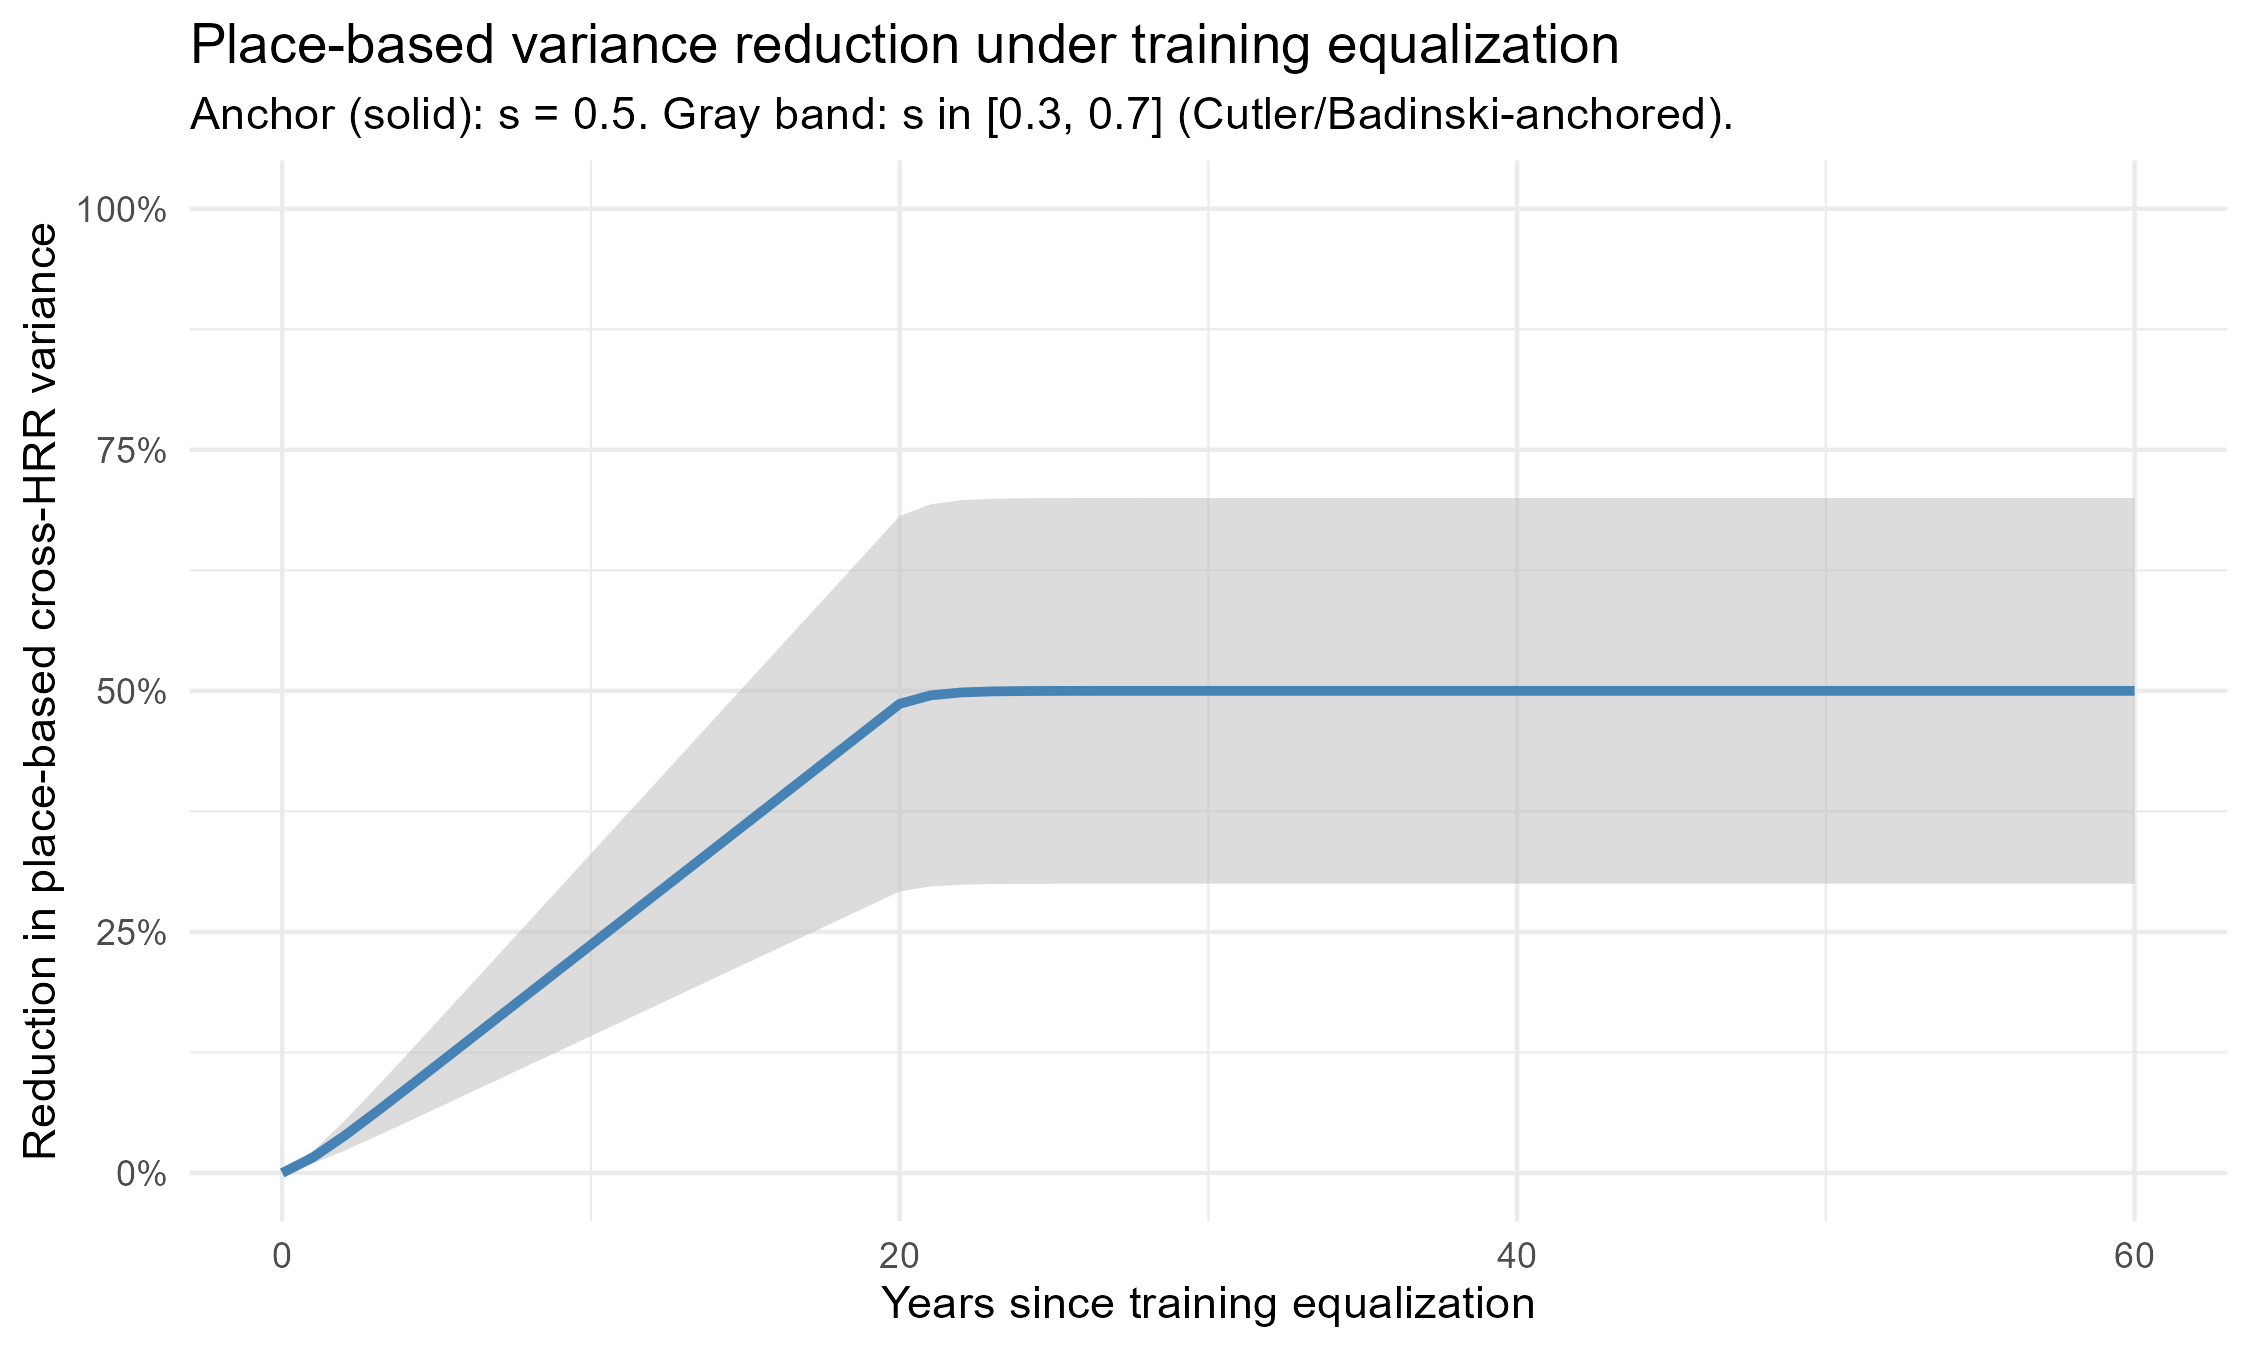
\includegraphics[width=\textwidth]{place-variance-path.png}
\end{minipage}
\end{figure}

The asymmetric persistence documented in the main paper applies to the variance-reduction path as well. An equalization regime that raises low-availability training HRRs to the national mean propagates more durably than one that lowers high-availability training HRRs, because the asymmetric malleability concentrates adaptation in the up-mover direction. The pooled simulation reported here averages over both directions and therefore understates the long-run reduction achievable by upward-only equalization while overstating the reduction achievable by downward-only equalization.

\clearpage

%%%%%%%%%%%%%%%%%%%%%%%%%%%%%%%%%%%%%%%%%%%%%%%%
\begin{singlespace}
\bibliographystyle{aer}
\bibliography{BibTeX_Library}
\end{singlespace}
%%%%%%%%%%%%%%%%%%%%%%%%%%%%%%%%%%%%%%%%%%%%%%%%

\end{document}
